% generated by experiments/make_tex_figures.py -- do not edit by hand
\begin{figure}[t]
\centering
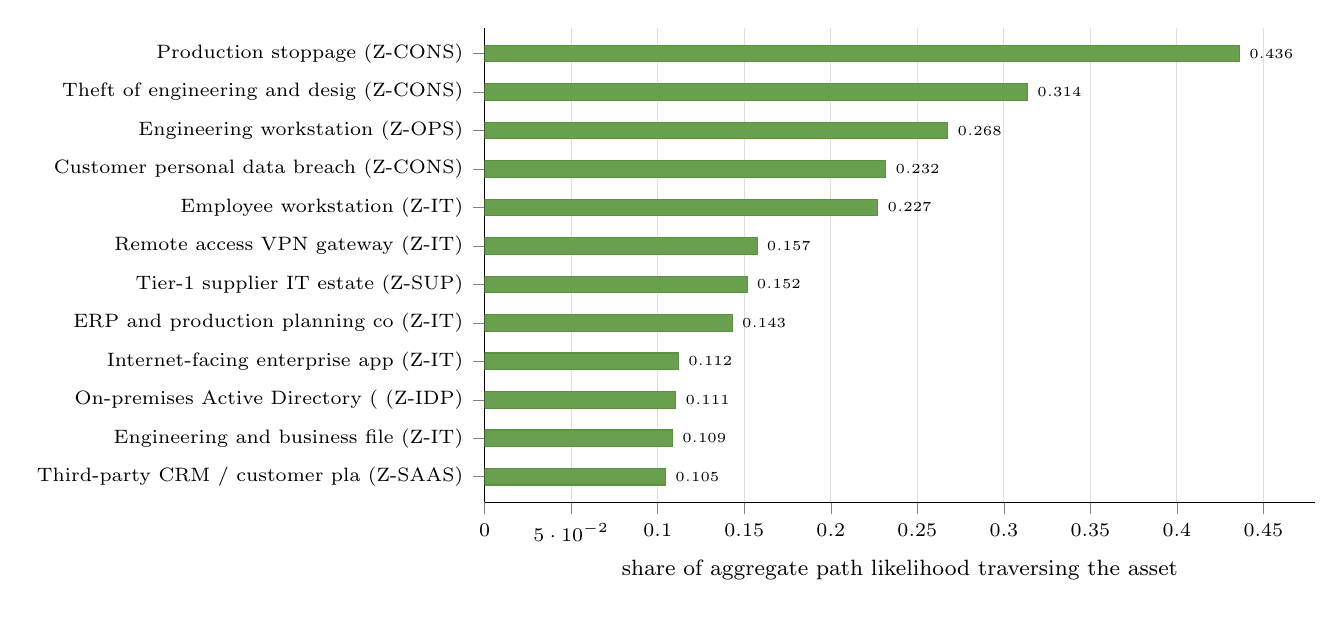
\begin{tikzpicture}
\begin{axis}[
    xbar, width=\linewidth, height=7.6cm,
    xlabel={share of aggregate path likelihood traversing the asset},
    xmin=0, enlarge y limits=0.06,
    ytick={0,1,2,3,4,5,6,7,8,9,10,11}, yticklabels={{Production stoppage (Z-CONS)},{Theft of engineering and desig (Z-CONS)},{Engineering workstation (Z-OPS)},{Customer personal data breach (Z-CONS)},{Employee workstation (Z-IT)},{Remote access VPN gateway (Z-IT)},{Tier-1 supplier IT estate (Z-SUP)},{ERP and production planning co (Z-IT)},{Internet-facing enterprise app (Z-IT)},{On-premises Active Directory ( (Z-IDP)},{Engineering and business file  (Z-IT)},{Third-party CRM / customer pla (Z-SAAS)}},
    y dir=reverse, ticklabel style={font=\scriptsize},
    label style={font=\footnotesize},
    nodes near coords, nodes near coords style={font=\tiny},
    every node near coord/.append style={/pgf/number format/fixed,
        /pgf/number format/precision=3},
    xmajorgrids, grid style={gray!25}, axis lines*=left,
    bar width=6pt, tick align=outside,
]
\addplot[fill=OliveGreen!70, draw=OliveGreen!80] coordinates {
        (0.436200,0)
        (0.313800,1)
        (0.267700,2)
        (0.231800,3)
        (0.227200,4)
        (0.157400,5)
        (0.151600,6)
        (0.143100,7)
        (0.112000,8)
        (0.110500,9)
        (0.108500,10)
        (0.104500,11)
};
\end{axis}
\end{tikzpicture}
\caption{Likelihood-weighted choke points of the reference architecture.}
\label{fig:chokepoints}
\end{figure}
